\documentclass[14pt,a4paper,oneside]{article}

\usepackage[utf8]{inputenc}   


\usepackage{amsmath,amsthm,amssymb,appendix,bm,mathrsfs,ctex,geometry,tcolorbox,fancyhdr,tikz,esint,appendix}


%% GB/T 7714 宏包 ---- 引文格式
\usepackage[sort&compress]{gbt7714}
\bibliographystyle{gbt7714-numerical}



\numberwithin{equation}{subsection}             %%%%%% 公式编号




\geometry{left=1.7cm, right=1.7cm, top=2.54cm, bottom=2.54cm}    %%%%% 页面尺寸
\linespread{1.5}                             %%%%% 行距1.5倍
\pagestyle{fancy}



%%    设置页眉页脚
\fancyhf{}
\renewcommand{\headrulewidth}{0.15mm}
\fancyhead[C]{文献阅读报告}                   %%%%%% 页眉
\fancyfoot[C]{\thepage}                      %%%%%% 页脚 页码
\setlength{\headheight}{15pt}


%%   设置各种链接颜色为黑色
\usepackage[colorlinks,
            linkcolor=black,
            anchorcolor=black,
            citecolor=black,
            urlcolor=black
            ]{hyperref}



%%   例子编号
\newcounter{example}
\counterwithin{example}{subsection}
\newcommand{\examplename}{Example}
\newcommand{\exampleTitle}[1]{%
\textbf{\refstepcounter{example}\examplename\theexample:#1}\par}


%%  插入图片配置
\usepackage{graphicx,subfigure}
\usepackage[]{caption2} %新增调用的宏包
\numberwithin{figure}{subsection}               %%%%%% 图片编号

\graphicspath{ {./Figure/} }            %%%%% 设置图片文件所在目录
\DeclareGraphicsExtensions{.pdf,.svg,.jpeg,.png,.jpg}     %%%%% 支持图片格式


%%    支持tikz作图
\usepackage{tikz}
\usetikzlibrary{backgrounds,arrows}


\usepackage{pgfplots}
\pgfplotsset{compat=1.15}
\usepackage{mathrsfs}


\title{\textbf{文献阅读报告 8\\Ultrafast nonlinear optics in gas-filled hollow-core photonic crystal fibers [Invited] 后半部分}}                           %%%%% 标题
\author{骆禹天}                                           %%%%% 作者
\date{2024/**/**}                                        %%%%%% 日期

%%   定义一些数学格式
\newtheorem{theorem}{定理}[subsection]
\newtheorem{definition}[theorem]{定义}
\newtheorem{lemma}[theorem]{引理}
\newtheorem{corollary}[theorem]{推论}
\newtheorem{example}[theorem]{例}
\newtheorem{proposition}[theorem]{命题}
\renewcommand{\abstractname}{\Large\textbf{摘要}}




%------------------------- 开始文档  -------------------------%



\begin{document}

\pagenumbering{Roman}         %%%%% 目录前页码统计按罗马数字

\maketitle

\setcounter{page}{1}          %%%%% 标题开始统计页数

%------------------------- 目录  ------------------------------%

\tableofcontents              %%%%% 插入目录

\newpage
\setcounter{page}{1}          %%%%% 目录后重新统计页数


\pagenumbering{arabic}        %%%%% 目录后统计页码为阿拉伯数字



%%%%%%%%%%%%%%%%%%%% 开始第一节  %%%%%%%%%%%%%%%%%%%%%



\section{脉冲压缩}

\subsection{光纤-光栅/啁啾镜压缩}

常见脉冲压缩技术两阶段: 

1. 自相位调制 (SPM) 非线性光谱展宽, 正色散; 

2. 反常色散压缩器 (光栅或啁啾镜) 补偿正色散. 

可设计PBG 引导 HC-PCF 为非常低非线性和强反常色散, 峰值功率$\sim$1 MW (由于非线性和光学损伤, 远高于实芯光纤的可能性) 下用来取代光栅/反射镜. 由于非线性远高于实芯光纤中的可能功率. 压缩过程中的影响和光学损伤的发生. 然而, 有限的传输带宽和较大的色散斜率限制了PBG 引导 HC-PCF在非线性光谱展宽阶段的使用. 

Kagomé PCF 具有宽导带、可调谐 GVD, GVD 斜率小, 可在两个阶段中有应用. 此外, kagomé PCF 的非线性介于实芯和空心毛细管之间, 能够在脉冲能量 (0.1-100 $\mathrm{\mu J}$) 下的非线性光谱展宽中使用, 此能量范围远低于毛细管, 但大大超过实心纤维能力. 

\subsubsection{设计实例}

图 \ref{p1.1.1} 显示了一潜在设计的数值模拟, 

· 输入: 10 $\mathrm{\mu J}$、30 fs 脉冲

· kagomé PCF, 芯直径为 70 $\mathrm{\mu m}$、填充有 43 bar 氩气

这导致 ZDW 移动到 1300 nm, 以便脉冲 (800 nm) 在正常色散区域中传播. 

观察到时间和光谱展宽, 正如正常色散和 SPM 组合所预期的那样. 图 \ref{p1.1.1}(b) 显示了传播 8 cm 后强度时域形状和平滑的抛物线时间相位. 该相位分布可以通过线性压缩器补偿. 

\begin{figure}[h]
    \centering
    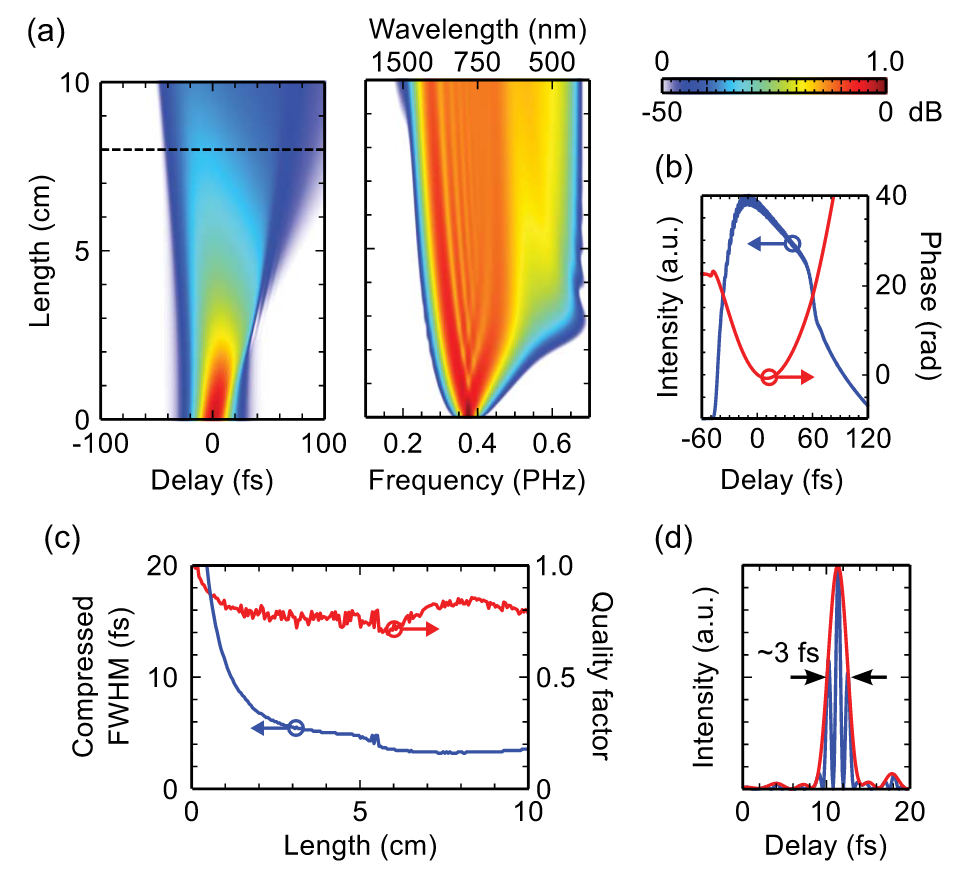
\includegraphics[width=0.4\textwidth]{p1.png}
    \caption{kagomé PCF 的光纤-光栅/镜面脉冲压缩;  (a) 脉冲通过 kagomé PCF 时间和光谱演化密度图, 将 ZDW 置于 1300 nm;  (b) 强度加宽时间形状, 以及在 kagomé PCF 中传播 8 厘米后的平滑抛物线时间相位 [(a) 中的虚线];  (c) 线性压缩后脉冲持续时间与用于谱展宽的 kagomé PCF 长度 (左轴) 和压缩品质因数 (右轴) ;  (d) (b) 线性压缩后的脉冲. }\label{p1.1.1}
\end{figure}

传播 8 cm后, 脉冲压缩至约 3 fs, 显示出非常干净的少周期电场, 峰值功率从 0.3 GW 增加到 3 GW. 

请注意, 最终的峰值功率不会出现在光纤内部而是在自由空间压缩阶段之后, 允许比充气 Kagomé PCF 内存在的峰值功率高得多. 

光纤-光栅压缩的质量使用品质因数来量化的, 品质因数定义为压缩脉冲的 1 FWHM 强度内的能量与未压缩脉冲的 1 FWHM 强度内包含的能量之比. 在图 \ref{p1.1.1}(d) 的示例中, 该因子超过 80\%, 事实上, 从图 \ref{p1.1.1}(c) (右轴) 可见, 在该特定系统设计中, 该因子从未低于 70\%. 

进一步的能量缩放可能需要使用正气体梯度. 由于气体压力较低, 在光纤输入端处的电离影响减少, 此处峰值强度最高. 随着脉冲在传播过程中暂时变宽, 强度会降低 [图 \ref{p1.1.1}(a)], 但采用正压力梯度, 可以实现一致的 SPM. 或者可使用向锥形 kagomé PCF 降低光纤输入端强度, 同时在整个传播过程中保持 SPM 展宽和正常色散. 

\subsection{孤子效应压缩}

另一种方案涉及孤子自压缩, 通常在实芯光纤中实现, 但非常适合 kagomé PCF. 

在此过程中, 反常色散和 SPM 的相互作用导致脉冲自压缩——高阶孤子传播的初始阶段. 在这一现象由 PBG 引导 HC-PCF 已成功证明, 可产生兆瓦峰值功率的脉冲, 超出了熔融石英的损伤极限.  Kagomé PCF 更具优势, 因为其固有的较弱高阶色散 (通常是极端脉冲压缩的限制因素) 及其更宽传输带宽. 

Joly 等人在探索在充满 Ar 的 kagomé PCF 中高效产生深紫外光时, 通过实验证明了孤子效应自压缩$\sim$30 fs 脉冲至短于 10 fs. \cite{lehmeierNonresonantThirdOrder1985}在这些实验中, PCF 比最佳压缩长度长得多. 数值模拟表明, 短至 4 fs 的脉冲一定发生在最大压缩位置, 与紫外线发射的开始时间一致. 

\subsubsection{压缩比和品质因数缩放}

通过大量数值模拟的详细分析\cite{mosleyUltrashortPulseCompression2010, dianovOptimalCompressionMultisoliton1986}, 最后得出以下关于孤子阶数的压缩比和品质因数的关系:
\begin{equation}
    F_c\thicksim4.6N,\quad\quad Q_c\thicksim3.7/N
    \label{eq:1.2.1}
\end{equation}

这意味着 800 nm 的 30 fs 脉冲可以被压缩到小于 N $\sim$ 3 的单个光周期. 这种极端压缩不可避免地受到高阶效应的限制, 例如高阶色散. 

图 \ref{p1.2.1} 显示了通过充 Ar 的 kagomé PCF (30 $\mathrm{\mu m}$ 芯直径) 数值结果. 

\begin{figure}[h]
    \centering
    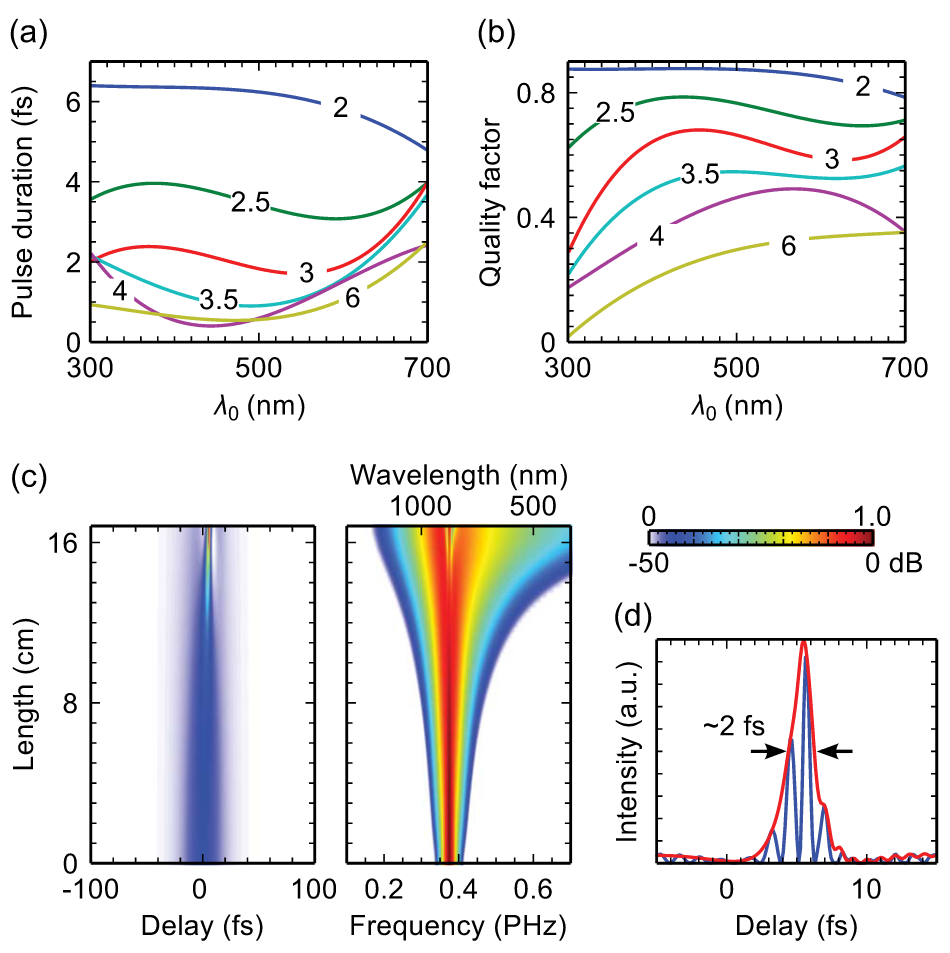
\includegraphics[width=0.4\textwidth]{p2.png}
    \caption{直径为 30 $\mathrm{\mu m}$ 充 Ar 的 kagomé PCF 中 800 nm 处孤子自压缩: (a) 压缩脉冲持续时间对 $\lambda_{0}$ (水平轴) 和 N (数字曲线) 的依赖性, (b)相应的品质因数依赖性, (c) $\lambda_{0} = 500 nm$、$N = 3.5$ 的脉冲自压缩的时域频域演化, 以及 (d) 最佳点处压缩输出脉冲场 (c) 中的压缩. }\label{p1.2.1}
\end{figure}


图 \ref{p1.2.1}(a) 显示了作为 ($\lambda_{0}$, N) 函数的最短自压缩脉冲持续时间. 随着 N 的增加, 压缩脉冲会变短, 直至在 N = 4 和 6 之间饱和. 压缩脉冲的持续时间与 $\lambda_{0}$ 的关系微弱; 当 $\lambda_{0}$ 接近泵浦波长 (800 nm) 时, 高阶色散开始扰乱自压缩, 导致过早的脉冲裂变. 随着 $\lambda_{0}$ 进一步远离 800 nm, 这需要较低的气压, 因此需要更高的泵浦强度, 气体开始发生电离, 从而降低自压缩过程的有效性. 

图 \ref{p1.2.1}(b) 显示了压缩脉冲品质因数与 ($\lambda_{0}$, N) 的函数关系. 如方程\ref{eq:1.2.1}, 随 N 增加, 这种情况会显着降低, 并且当 $\lambda_{0}$ 远离 800 nm 时也会降低. 

压缩脉冲持续时间和品质因数之间存在权衡. 一个好的选择是 $\lambda_{0}$ = 500 nm, N = 3.5; 这些参数的 30 fs 脉冲的频谱和时间演变如图 \ref{p1.2.1}(c) 所示. 与正常色散状态下传播相反[图\ref{p1.1.1}(a)], 可看出时间轮廓传播时急剧锐化. 在最佳压缩点, 会产生约 2 fs 的脉冲 [图\ref{p1.2.1}(c)]. 对于较高的 N 值 ($\sim$9), 自压缩脉冲可达到少周期持续时间, 但质量显着下降, 且脉冲光谱扩展到 UV 范围. 紫外色散波的发射由此开始. 

\subsubsection{较长脉冲的影响}

如果我们增加泵脉冲持续时间, 压缩会发生什么？

从方程\ref{eq:1.2.1}, 可将压缩脉冲持续时间$\tau_{c}$写为: 
\begin{equation}
    \tau_c=\frac{\tau_0}{F_c}\propto\frac{\tau_0}N\propto\sqrt{\frac{|\beta_2|}{\gamma P_0}}
    \label{eq:1.2.2}
\end{equation}

这表明如果泵浦脉冲的峰值功率保持不变, 则 $\tau_{c}$保持不变; 即孤子阶数与脉冲持续时间 $\tau_{0}$ 成比例增加.然而, 方程\ref{eq:1.2.1}表明, 品质因数随着孤子阶数的增加而显着降低, 导致随着 $\tau_{0}$ 变长而导致更差的压缩.

\subsubsection{绝热脉冲压缩}

绝热孤子压缩\cite{kuehlSolitonsAxiallyNonuniform1988, traversOpticalPulseCompression2007, traversOpticalPulseCompression2007}也已在锥形PBG引导HC-PCF中得到证实\cite{geromeDeliverySub100fsPulses2007}.数值分析表明, 如果施加压力梯度以使GVD随着传播距离而减小, 则可以达到最短的脉冲持续时间\cite{laegsgaardTheoryAdiabaticPressuregradient2009}, 从而避免了使纤维结构本身逐渐变细的需要.模拟还表明, 降低色散和孤子效应压缩的结合可以实现更高的压缩比, 而不会损害品质因数.

Kagomé PCF 可用于绝热压缩, 正压力梯度会导致 $\gamma$ 增加和 $\beta_{2}$ 减少, 非常适合此过程.然而如果要保持绝热压缩, 光纤长度必须是色散长度的许多倍, 因此该技术仅限于最短的输入脉冲持续时间, 因为最佳情况下的损耗约为 0.3 dB/m 限制可用光纤长度可达$\sim$10 m.

\section{紫外中色散波的产生}

可使用充 Ar 的 kagomé PCF 产生高效的深紫外光, 发射的紫外线波长可通过改变气压和色散来调节.

图 \ref{p2.0.1}(a) 显示了一系列实验获得 UV 光谱: 

· 输入: 在 800 nm 下以 45 fs 脉冲泵浦

· 直径 27 $\mathrm{\mu m}$ 的充 Ar kagomé PCF.

· 调节脉冲能量 (0.5-3 $\mathrm{\mu J}$) 和充气压力 (4-12 bar) 来获得的, 以证明清洁 UV 输出的可调范围为 200-300 nm.光谱的相对宽度为$\sim$0.03.

\begin{figure}[h]
    \centering
    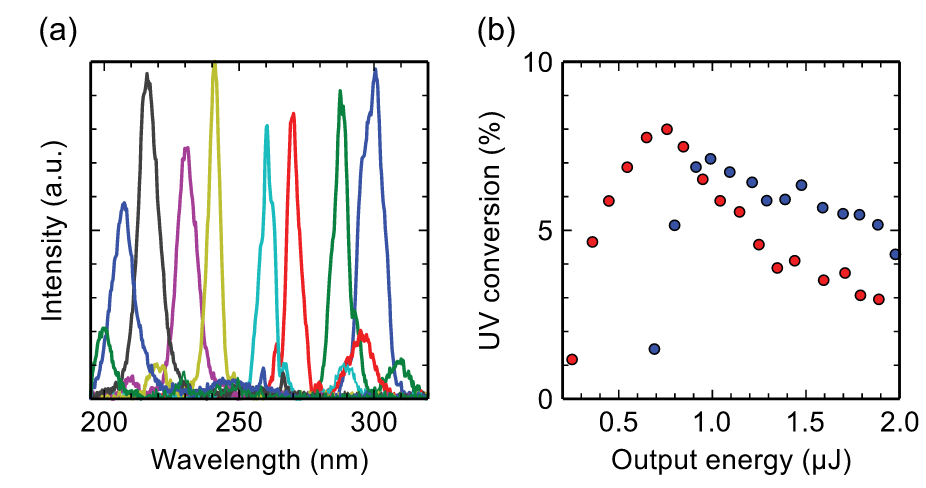
\includegraphics[width=0.4\textwidth]{p3.png}
    \caption{深紫外色散波产生;  (a) 从充满 Ar 的 27 $\mathrm{\mu m}$ 芯直径 kagomé PCF 中通过实验获得的一系列可调谐输出光谱  (800 nm 处的 45 fs 脉冲, 0.5-3 $\mathrm{\mu J}$ 脉冲能量和 4-12 bar 气压)  (b) 报告的紫外线转换效率\cite{jolyBrightSpatiallyCoherent2011}.}\label{p2.0.1}
\end{figure}

图 \ref{p2.0.1}(b) 显示了 Jolly等人的工作\cite{jolyBrightSpatiallyCoherent2011} 中, 通过实验实现的 UV 转换效率, 其中在较宽的功率调谐范围内测得 6\% 至 8\% 的转换率, 表明 kagomé PCF 的 UV 输出能量约为 50-80 nJ,$\lambda_{0}$$\sim$600 nm, N $\sim$ 9.

\subsection{色散波的相位匹配}

kagomé PCF 紫外光的产生是由输入脉冲的极端孤子效应脉冲压缩引起的, 与共振色散波频率重叠的光谱扩展, 因此被激发\cite{waiNonlinearPulsePropagation1986, waiRadiationsSolitonsZero1990, karpmanRadiationSolitonsDue1993, imHighpowerSolitoninducedSupercontinuum2010}.孤子在其中心频率附近是稳定的, 因为它们以比相同频率的色散波更高的相速度传播.然而, 在存在高阶色散的情况下, 它们可以与其他频率的色散波进行相位匹配; 即 $\beta(\omega)=\beta _{\mathrm{sol}}(\omega)$, 其中 $\beta (\omega)=n_{mn}k$ 是线性模式传播常数, 并且
\begin{equation}
    \beta_{\mathbf{sol}}(\omega)=\beta(\omega_{\mathbf{sol}})+\beta_1(\omega_{\mathbf{sol}})[\omega-\omega_{\mathbf{sol}}]+\frac{\gamma P_c}2
    \label{eq:}
\end{equation}
其中 $P_c$ 是自压缩脉冲峰值功率, $ω_{sol}$ 是孤子频率.在图 11(a) 中, 我们绘制了直径 30 $\mathrm{\mu m}$ 的 kagomé PCF 中一系列 Ar 压力的传播常数失配 $[\beta(\omega)-\beta(\omega_{\mathbf{sol}})]$.可见相位匹配点出现在紫外光谱区域.由于 $P_c\approx P_0F_c$ , 并围绕 $\omega_{sol}$ 扩展开 $\beta (\omega)$, 相位匹配条件简化为
\begin{equation}
    \sum_{n\geq2}\frac{(\omega-\omega_{\mathbf{sol}})^n}{n!}\beta_n(\omega_{\mathbf{sol}})=\frac{\gamma P_c}2\thicksim2.3\gamma P_0N
    \label{eq:2.1.2}
\end{equation}

在图 \ref{p2.1.1}(b) 和 \ref{p2.1.1}(c) 中, 将两个不同系统 (直径为 10 $\mathrm{\mu m}$ 充 Xe 系统和直径为 50 $\mathrm{\mu m}$ 充 He 的 kagomé PCF) 的相位匹配条件绘制为 ($\lambda_0$, N) 的函数.对于 800 nm 泵浦脉冲, 至少可以在 150 至 500 nm 范围内找到相位匹配的解决方案.虽然对 $\lambda_0$ (以及气压) 的依赖性很强, 但在 UV 区域, 对 N 的依赖性相对较弱, 尽管当 $\lambda_0$ 接近 800 nm 时, 它变得更加显着, 并且对方程
\begin{equation}
    n_{mn}(\lambda,p,T)=\sqrt{n_{\mathrm{gas}}^2(\lambda,p,T)-\frac{u_{mn}^2}{k^2a^2}}\simeq1+\delta(\lambda)\frac p{2p_0}\frac{T_0}T-\frac{u_{mn}^2}{2k^2a^2},
    \label{eq:}
\end{equation}
的非线性贡献也变得更加显着. 方程 \ref{eq:2.1.2} 变得更加占主导地位.这两个图之间十分相似, 仅在 150 nm 左右的极端相位匹配中才发现明显的分歧, 此时高阶色散变得很重要

\begin{figure}[h]
    \centering
    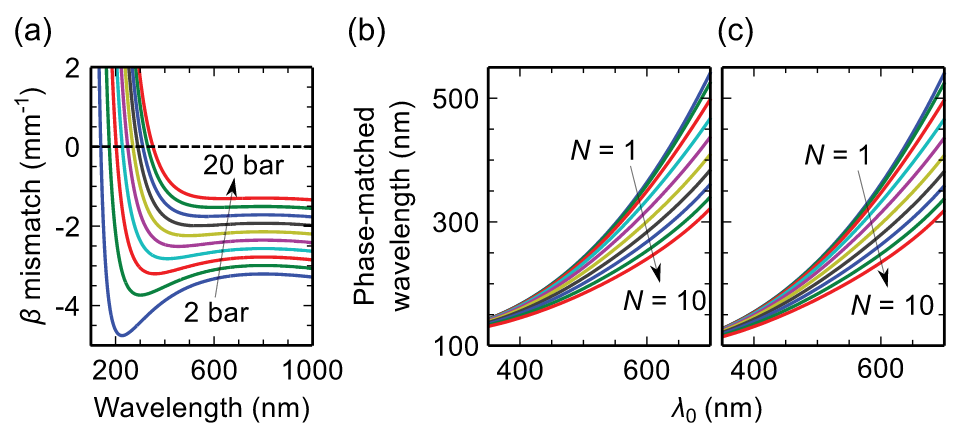
\includegraphics[width=0.4\textwidth]{p4.png}
    \caption{(a) 对于填充有 2 至 20 bar Ar 的 30 μm kagomé PCF (2 bar 步长) , 孤子 (800 nm 处的 N 1⁄4 9) 和色散波在给定波长下的传播常数不匹配;  (b)、(c) (b) 10 $\mathrm{\mu m}$ 直径充 Xe 光纤和 (c) 50 $\mathrm{\mu m}$ 直径充 He 光纤的相位匹配波长, 假设压力可调谐 ZDW $\lambda_{0}$}\label{p2.1.1}
\end{figure}

\subsection{深紫外产生的效率}

色散波产生的效率很大程度上取决于相位匹配频率下压缩脉冲的频谱功率密度. 因此, 如果初始泵浦光谱要扩展到紫外区域, 那么严格的时间自压缩至关重要.在kagomé PCF系统中, 自陡峭和光学激波形成, 不对称地增强SPM展宽光谱的蓝色边缘, 是增强这一过程的关键.

输入脉宽有什么影响？

在图\ref{p2.2.1} (a) 中可见, 无论脉冲持续时间和泵浦能量范围如何, UV 转换效率 (波长短于 350 nm 的总功率分数) 都是可能的.使用因子 $Q_\mathrm{UV}=P_\mathrm{FWHM}/P_\mathrm{UV}$ 量化 UV 发射的质量, 其中 $P_\mathrm{FWHM}$ 是最强 UV 峰值的 FWHM 内的光谱功率, $P_\mathrm{UV}$ 是 UV 区域中的总光谱功率.

图 \ref{p2.2.1}(b) 显示 $Q_\mathrm{UV}$ 强烈依赖于泵浦脉冲持续时间.对于 15 fs, 对于各种泵参数, 超过 90\% 的 UV 功率位于主 UV 峰值, 而 120 fs 脉冲的这一比例不到 30\%.

这在图 \ref{p2.2.1}(c) 中非常明显, 该图显示了 15、30、60 和 90 fs 脉冲沿光纤的光谱演化, 标准化孤子阶数为 $\mathrm{CS}=N/\tau_{\mathrm{FWHM}}=0.26$ (对于 30 fs 脉冲持续时间 N = 7.8) .对于 15 fs 脉冲, 大约在孤子裂变长度处出现高质量的 UV 波段.

\begin{figure}[h]
    \centering
    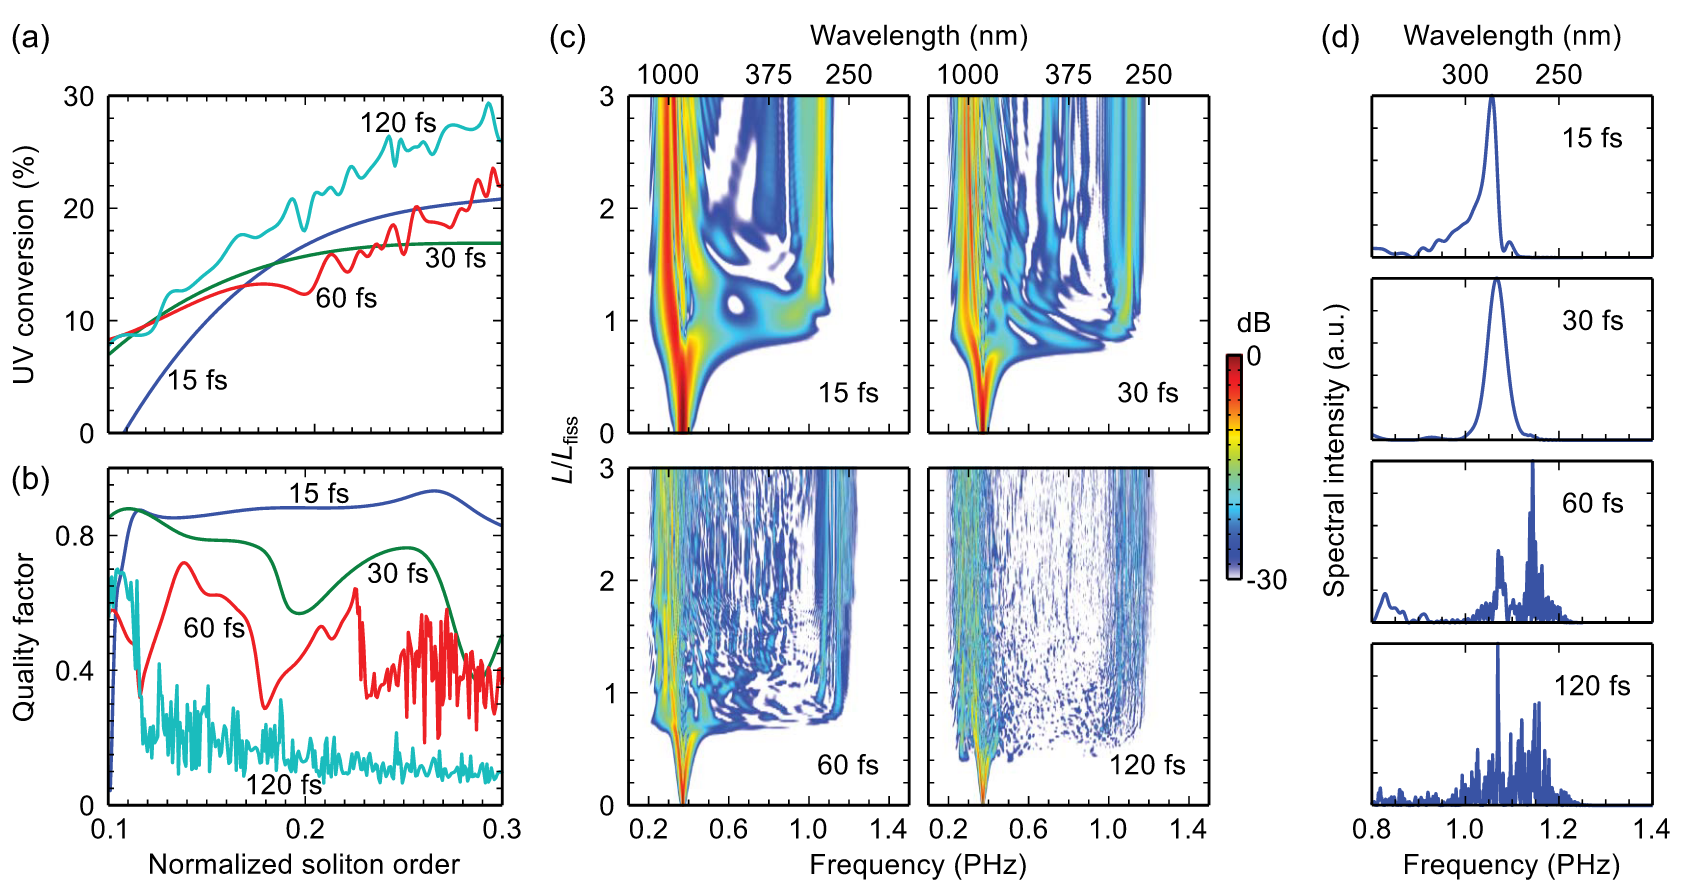
\includegraphics[width=0.8\textwidth]{p5.png}
    \caption{UV 产生对脉冲持续时间 (15、30、60 和 120 fs) 和 $\lambda_{0}$ = 600 nm 光纤孤子阶次的依赖性 (kagomé PCF, 具有 30 $\mathrm{\mu m}$ 芯直径, 填充 9.8 bar Ar) : (a)紫外转换效率 (波长短于 350 nm) 作为归一化孤子阶次 $S = N=τ_{\mathrm{FWHM}}$ 的函数, 对应于 30 fs 脉冲的 N = 3 至 9;  (b) 对于与 (a) 相同的参数, 文本中定义的 UV 转换品质因数;  (c) S = 0.26 处每个脉冲持续时间沿光纤的光谱演变;  (d) 每个脉冲持续时间的最佳 UV 转换位置处的光谱切片.}\label{p2.2.1}
\end{figure}

对于 30 fs 泵浦, UV 波段仍然具有相对较高的质量, 但在 60 fs 时, 它会显着降低, 而在 120 fs 时, 可以观察到 MI 的证据 - UV 波段形成相当精细的结构, 如在图\ref{p2.2.1}(d)中的光谱切片.这种质量下降的原因是高 N 值时脉冲自压缩的品质因数降低.要以高转换效率获得高质量的 UV 光谱, 需要$\sim$30 fs 或更短的脉冲持续时间.如果我们降低峰值功率, 则可以使用更长的脉冲实现高质量转换, 但效率会显着降低.

发射的紫外光在产生时可能是几个光学周期, 但它在正常色散区域中传播, 导致群速度展宽.然而, kagomé PCF 相对平坦且简单的色散特性应使在光纤输出端对啁啾 UV 脉冲进行外部压缩变得简单.甚至可以通过真空 kagomé PCF 传播来实现压缩, 该 PCF 在所有波长上都具有反常色散.

\subsection{紫外超连续谱产生}

通过发射例如 10 $\mathrm{\mu J}$ 600 fs 脉冲将孤子阶数提高到 N $\sim$ 245, 使系统很好地进入 MI 状态, 可以预期这会得到平滑且广泛的超连续谱生成.

为了说明这一点, 图 \ref{p2.3.1} 显示了如此长的脉冲在 $\lambda_{0}$ = 750 nm (25 bar Ar, 30 $\mathrm{\mu m}$ 直径) 的 kagomé PCF 中的传播.图 \ref{p2.3.1}(a) 显示了一次发射的时间演化, 图 \ref{p2.3.1}(b) 显示了 30 次模拟的整体平均值的光谱演化 (在 MI 体系中, 每个激光发射产生不同的光谱, 通过包含量子噪声进行建模, 并对多次拍摄进行平均) .在时间图中, 可以清楚地观察到输入脉冲分裂成大量超短孤子, 随后经历多次碰撞.在光谱域中, 这会产生跨越 350 至 1500 nm 范围的平滑、平坦、高能超连续谱.请注意, 在没有拉曼散射的情况下, MI 超连续谱显示出蓝色增强的不对称性, 这与玻璃芯光纤中看到的情况相反.

\begin{figure}[h]
    \centering
    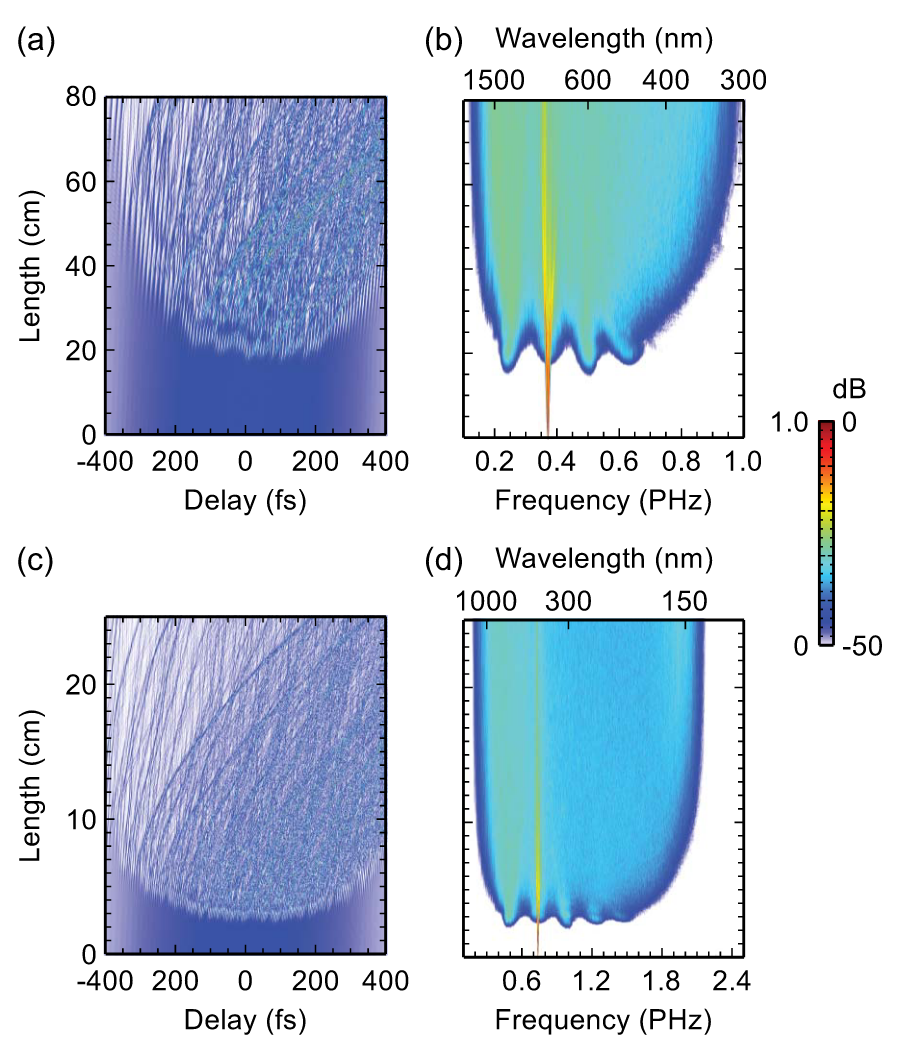
\includegraphics[width=0.4\textwidth]{p6.png}
    \caption{(a), (b) 在 $\lambda_{0}$ = 750 nm 的 kagomé PCF 中以 800 nm 传播 N $\sim$ 245 (600 fs, 10 $\mathrm{\mu J}$) 脉冲 (30 $\mathrm{\mu m}$ 芯直径, 填充 25 bar Ar) :  (a)一次发射的时间演化和 (b) 30 次模拟的整体平均值的光谱演化. (c), (d) 在 kagomé PCF 中以 400 nm 传播 N $\sim$ 429 (600 fs, 10 $\mathrm{\mu J}$) 脉冲, 波长为 $\lambda_{0}$ = 350 nm (芯直径为 10 $\mathrm{\mu m}$, 填充有 8.8 bar Ar)  : (c) 单次时间演化和 (d) 30 次模拟的整体平均值的光谱演化.}\label{p2.3.1}\end{figure}

将 kagomé PCF 中的 ZDW 调整到 UV 使得能够将这些动力学机制转移到更短的波长.例如, 如果我们使用与上述相同的参数进行泵浦, 但在设计用于 350 nm 零色散 (8.8 bar Ar, 10 $\mathrm{\mu m}$ 纤芯直径) 的光纤中的泵浦波长为 400 nm, 可以得到非常平坦且光滑、基于 MI 的高能超连续谱, 延伸范围为 140-1000 nm [图 \ref{p2.3.1}(c)和(d)]; 这种系统的实验实现将为计量学和光谱学提供独特的来源.









%--------------------  插入参考文献  --------------------%

\newpage

\clearpage           %%%  “目录”中显示的页码正确, 需要添加 \clearpage
\phantomsection      %%   “目录”中的链接能正确跳转, 需要添加 \phantomsection
\addcontentsline{toc}{section}{参考文献}   %向目录中添加条目, 以章的名义

\bibliography{ref}

\end{document}